\documentclass[12pt,a4paper,UTF8]{ctexbook}
\usepackage[top=2cm, bottom=2cm, left=2cm, right=2cm]{geometry} % 页边距
\usepackage{amsmath,amssymb}    % 数学公式
\usepackage{graphicx}           % 图片插入
\usepackage{booktabs}           % 专业表格
\usepackage{multirow}            % 表格跨行
\usepackage{amsthm}
\usepackage[colorlinks=true]{hyperref} % 超链接
\usepackage{tikz}
\usepackage{pgfplots}

%自定义宏
%公式命令宏
\theoremstyle{plain}
\newtheorem{theorem}{\indent Theorem}[section]
\newtheorem{lemma}[theorem]{\indent Lemma}
\newtheorem{proposition}[theorem]{\indent Proposition}
\newtheorem{corollary}[theorem]{\indent 推论}
\newtheorem{definition}{\indent Definition}[section]
\newtheorem{example}{\indent Example}[section]
\newtheorem{remark}{\indent Remark}[section]
\newenvironment{solution}{\begin{proof}[\indent\bf Solution]}{\end{proof}}
\newtheorem{axiom}{\indent Axiom}[section]
\renewcommand{\proofname}{\indent\bf Proof}
% 快速输入数学符号
\newcommand{\R}{\mathbb{R}}    % 实数集
\newcommand{\C}{\mathbb{C}}    % 复数集
\newcommand{\Z}{\mathbb{Z}}    % 整数集
\newcommand{\Q}{\mathbb{Q}}    % 有理数集
\newcommand{\N}{\mathbb{N}}    % 自然数集

% 微分符号 (直立体)
\newcommand{\diff}{\mathop{}\!\mathrm{d}} % 用法: \int f(x) \diff x

% 概率期望/方差
\newcommand{\E}{\mathbb{E}}    % 期望
\newcommand{\Var}{\operatorname{Var}}    % 方差

% 自动调整括号大小
\newcommand{\paren}[1]{\left(#1\right)}   % 圆括号
\newcommand{\bracket}[1]{\left[#1\right]} % 方括号
\newcommand{\braces}[1]{\left\{#1\right\}} % 花括号

% 向量/矩阵(粗体)
\newcommand{\vb}[1]{\mathbf{#1}}          % 向量 \vb{v}
\newcommand{\mat}[1]{\mathbf{#1}}         % 矩阵 \mat{A}
\newcommand{\tran}{^{\mathsf{T}}}         % 转置 A\tran

\usetikzlibrary{3d}
\pgfplotsset{compat=1.18}
\usepgfplotslibrary{colormaps}

\title{Learning Calculus with Linear Algebra}        
\author{hotteano\\
        南方科技大学}
\date{\today }
\begin{document}

\maketitle
\tableofcontents

\chapter{集合论与实数构造}  
\section{数集与映射}
\subsection{策梅洛-弗兰克尔集合论公理体系}
\begin{axiom}[外延公理]
    \begin{equation}
        \forall P \forall Q \left( \forall x (x\in P \Leftrightarrow x\in Q) \leftrightarrow  P=Q \right)
    \end{equation}
\end{axiom}


\section{确界原理}
\section{极限的定义}
\section{闭区间套定理}
\section{有限覆盖定理}
\section{数列极限}

\section{柯西列与柯西收敛原理}
\section{上下极限}
\subsection{上极限}uu
(数列的上极限)首先令部分柯西列的上确界$a^{+}_N:=\sup(a_n)^\infty_{n=N}$,接着定义柯西列$(a_N^{+})^\infty_{N=m}$,利用此,定义上极限: $\overline{\lim_{n\to\infty}}a_n:=\lim \underset{n\to \infty}{\sup}a_n=\inf (a_N^{+})^\infty_{N=m}$
\section{分段估计技术}
部分和极限存在的充要条件是,存在一个$N$,使得对于$n>N$的都有$S=\sum_{n=N+1}^\infty a_n$收敛,那么原部分和数列$S_n=\sum_{n=1}^N a_n+\sum_{n=N+1}^\infty a_n$收敛。
\chapter{函数的极限}
\section{函数极限的定义}
对于一个函数$f(x)$,在某点$(x_0,f(x_0))$的极限定义为:对于任意$\epsilon>0$与一个常数$A$存在某个去心邻域$(x_0-\delta,x_0+\delta)$,对于这个邻域中的所有$f(x)$,都有$|f(x)-A|<\epsilon$,我们称$A$为$f(x)在x=x_0$处的极限。
\section{极限的运算法则}

\section{求函数极限的常见方法}
\section{等价无穷小}
\section{求极限初等代数变形技巧}
\section{夹逼准则}
\section{单边极限}
\section{连续性}
\section{间断点}
\section{介值定理}
\section{渐近线及其求法}
\section{一致连续}

\chapter{微分与导数}
\section{导数}
\section{极值点}
\section{可微与连续}
\section{隐函数求导}
\section{反函数的导数}
\section{中值定理}
\section{作图方法}
\section{线性近似}
\section{牛顿法}


\chapter{积分}
\section{黎曼积分}
\section{积分中值定理}
\section{微积分基本定理}
\section{定积分的性质}
\section{旋转体的计算}
\section{反三角函数及其微积分性质}

\chapter{不定积分与定积分技巧}
\section{初等变换}
\section{换元积分}
\section{分部积分}
\section{有理函数积分与因式分解}
\section{组合积分}
\section{欧拉公式积分}
\section{递推积分}
\section{幂级数积分}
\section{双元法}
\section{无初等表示的判定}
\section{数值积分}

\chapter{线性方程组与矩阵}
\chapter{线性空间与线性映射}

\chapter{微分方程}
\section{常微分方程的通解与特解}
\section{欧拉法}
\section{龙格-库塔方法}
\section{一阶线性常微分方程}
\section{二阶线性常微分方程}
\section{自治微分方程}

\chapter{反常积分}
\section{反常积分的定义}
\paragraph{}第一类反常积分:对于积分$I=\int_a^\infty f(x)\mathrm{d}x=\lim_{x\to \infty}\int_a^xf(x)\mathrm{d}x.$若极限在任意区间上存在,称$I$收敛.
\paragraph{}第二类反常积分:对于积分$I=\int_a^b f(x)\mathrm{d}x$,$f(x)$在积分区间上存在无穷间断点。收敛条件同上。
\section{p积分}
\begin{equation}
    \int_{1}^\infty \frac{1}{x^p}\mathrm{d}x=\left\{ \begin{array}{lc}\frac{1}{1-p}&p\geq1\\diverge&0<p<1\end{array} \right.
\end{equation}
\paragraph{}
\begin{equation}
    \int_{0}^1 \frac{1}{x^p}\mathrm{d}x=\left\{ \begin{array}{lc}diverge&p\geq1\\\frac{1}{p-1}&0<p<1\end{array} \right.
\end{equation}
\section{瑕积分}
\section{反常积分的审敛法}
\subsection{比较审敛法}
\begin{theorem}
对于反常积分$I=\int^{\infty}_af(x)\mathrm{d}x$,如果函数$f(x)\geq g(x)$,在$(a,\infty)$上恒成立,$g(x)$
反常积分发散,那么其反常积分发散。如果$f(x)\leq g(x)$,在$(a,\infty)$上恒成立,$g(x)$
反常积分收敛,那么反常积分收敛。特别地,利用p积分的收敛性质,对于反常积分$I=\int^{\infty}_af(x)\mathrm{d}x$,如果函数
$f(x)\geq\frac{M}{x}$在$(a,\infty)$上恒成立,那么其反常积分发散。如果$f(x)\leq\frac{M}{x^p}$(其中$p>1$)在$(a,\infty)$
上恒成立,那么反常积分收敛。
\end{theorem}
\subsection{极限审敛法}
\begin{theorem}
若$\lim \frac{f(x)}{g(x)}=L,0<L<\infty$,那么反常积分$\int_a^\infty f(x)\mathrm{d}x$和$\int_a^{\infty}g(x)\mathrm{d}x$敛散性相同。
同理,可以利用与p积分比较判断积分的敛散性。\end{theorem}
\begin{remark}对于一个函数$Q(x)$具有的一系列函数因子$P_k(x)$,不妨取最大的函数因子$P_{\max}(x)$,再作商取极限。    
\end{remark}
\subsection{柯西审敛法(根值审敛法)}
\begin{theorem}
若函数在$(1,\infty)$上连续,若存在$q>0$,$\sqrt[x]{f(x)}\leq q<1$,那么反常积分$\int_{1}^{\infty}f(x)\mathrm{d}x$收敛。
\end{theorem}
\subsection{狄利克雷审敛法}
\begin{theorem}
对于反常积分$\int_a^\infty f(x)g(x)\mathrm{d}x$,如果$F(\alpha)=\int_{a}^\alpha f(x)\mathrm{d}x$在$(a,\infty)$有界,$g(x)$单调,$\lim_{x\to\infty}g(x)=0$,那么反常积分收敛。
\end{theorem}
\section{Gamma函数}
\begin{definition}
定义Gamma函数
\begin{equation}
\Gamma (z)=\int_{0}^\infty t^{z-1}e^{z}\mathrm d t. 
\end{equation}
$\Gamma$函数具有递推性质:$\Gamma(n+1)=n\Gamma(n)$,这表明$\Gamma(n)=n!$,当n为正整数。
\end{definition}
\begin{example}积分$I=\int_{0}^{\infty}e^{-x^2}\mathrm d x$与$\Gamma(n)$\end{example}
\begin{solution}注意到不妨令$x=y^{\frac{1}{n}}$,则$\mathrm d x=\frac{1}{nx^{n-1}}\mathrm dy$,从而$n\Gamma(n)=\int_{0}^\infty e^{-y^\frac{1}{n}}\mathrm d y$,

令$n=\frac{1}{2},\frac{1}{2}\Gamma (\frac{1}{2})=\int_{0}^\infty e^{-x^2}\mathrm{d}x$
\end{solution}
\begin{theorem}[余元公式]
\begin{equation}
\Gamma(1-z)\Gamma(z)=\frac{z}{\sin \pi z}
\end{equation}
\end{theorem}
\begin{proof}
    \begin{align*}
    LHS&=\int_0^\infty\frac{s^{z-1}}{1+x}\mathrm ds&\\&=\int_0^1\frac{s^{z-1}}{1+x}\mathrm ds+\int_1^\infty \frac{s^{z-1}}{1+x}\mathrm ds&\\
    &=\int_0^1\frac{s^{z-1}}{1+x}\mathrm ds+\int_0^1 \frac{s^{-z}}{1+z}\mathrm ds&\\&=\sum_{k=0}^{\infty}(-1)^k\frac{1}{k+z}+\sum_{k=1}^{\infty}(-1)^k\frac{1}{k-z}&
    \end{align*}
注意到\begin{align*}\sum_{k=1}^\infty(-1)^k\frac{2\cos kx}{k^2-a^2}=\frac{1}{a^2}-\frac{\pi\cos ax}{a\sin a\pi}\end{align*}代入$x=0,a=z$,两侧同乘以z:
\begin{align*}\sum_{k=0}^{\infty}(-1)^k\frac{2z}{z^2-k^2}+\frac{1}{z}=\frac{\pi}{\sin\pi z}\end{align*}
\end{proof}
\section{Beta函数}
\begin{definition}
定义Beta函数
\begin{equation}
    B(x,y)=\int_0^1(1-t)^{x-1}t^{y-1}\mathrm{d}t 
\end{equation}
\end{definition}
\begin{remark}
其中不难注意到对称性$B(x,y)=B(y,x)$。注意到前面我们介绍的Gamma函数,很容易发现一个恒等式$B(x,y)=\frac{\Gamma(x)\Gamma(y)}{\Gamma(x+y)}$,
利用余元公式我们发现$B(1-z,z)=\Gamma(1-z)\Gamma(z)=\frac{\pi}{\sin \pi z}$。
\end{remark}
\section{罗巴切夫斯基函数}
\begin{definition}
定义罗巴切夫斯基函数:
\begin{equation}
    L(x)=-\int_0^x\ln(\cos t)\mathrm d t
\end{equation}
\end{definition}
\begin{remark}
对于该函数的估计,我们有级数展开:
\begin{equation}
    L(x)=x\ln2 -\frac{1}{2}\sum_{k=1}^\infty(-1)^{k-1}\frac{\sin 2kx}{k^2}
\end{equation}
\end{remark}
\section{狄利克雷积分}
\begin{equation}
    \int_0^\infty \frac{\sin x}{x}\mathrm d x=\frac{\pi}{2}
\end{equation}
\section{欧拉-泊松积分}
\begin{equation}
    \int_0^\infty e^{x^2}\mathrm d x=\frac{\sqrt{\pi}}{2}
\end{equation}
\section{菲涅尔积分}
\begin{equation}
    \int_0^\infty \sin x^2\mathrm d x=\int_0^\infty \cos x^2\mathrm d x=\sqrt{\frac{\pi}{2}}
\end{equation}
\section{拉普拉斯积分}
\begin{equation}
    \begin{split}
        L=\int_0^\infty \frac{\cos bx}{a^2+x^2}\mathrm d x=\frac{\pi}{2a}e^{-ab}\\
        K=\int_0^\infty\frac{x\sin bx}{a^2+x^2}\mathrm d x=\frac{\pi}{2}e^{-ab}
    \end{split}
\end{equation}
\section{欧拉积分}
\begin{equation}
    \int_0^\infty \frac{x^{a-1}}{1+x}\mathrm d x=\frac{\pi}{\sin \pi a},0<a<1
\end{equation}
\section{伏汝兰尼积分}
\begin{equation}
    \int_0^\infty\frac{f(ax)-f(bx)}{x}\mathrm d x=(f(0)-f(+\infty))\ln\frac{b}{a}
\end{equation}

\chapter{级数}
\section{级数}
\subsection{常数项级数}
常数项级数:给定数列$a_n$,定义其部分和数列$S_n=\sum_{i=1}^na_i$,那么称$\lim_{n\to \infty}S_n=\sum_{i=1}^\infty a_i$为(常数项)级数
\subsection{交错级数}
交错级数:给定数列$a_n$,定义$\lim_{n\to\infty}S_n=a_1-a_2+a_3-\cdots=\sum_{i=1}^\infty (-1)^{i+1}a_i$为交错级数。
\subsection{函数项级数}
函数项级数:函数列部分和极限$\lim_{n\to\infty}\sum_{i=1}^nu_i(x)=\sum_{i=1}^\infty u_i(x)$称为(函数项)级数。例如泰勒级数。
\section{级数的收敛性}
若数列部分和数列极限收敛,则级数收敛;若极限不存在,称之为发散。对于上述的交错级数和常数项级数,我们定义以下两个收敛概念:
\paragraph{}(1)绝对收敛:对于级数$\sum_{n=1}^\infty u_n,\sum_{n=1}^\infty|u_n|$收敛,则称级数绝对收敛。级数绝对收敛是级数收敛的充分条件.
\paragraph{}(2)条件收敛:对于级数$\sum_{n=1}^\infty u_n,\sum_{n=1}^\infty|u_n|$不收敛,而$\sum_{n=1}^\infty u_n$收敛,则称级数条件收敛。
\paragraph{}以下是绝对收敛数列的良好性质:
\paragraph{}1.绝对收敛数列改变项位置后的新级数与原级数收敛于同一值;
\paragraph{}2.定义第$k-1$项柯西乘积$\sum_{i=1}^k(u_nv_{n-i})$.则级数的柯西乘积
$\sum_{n=1}^\infty u_n\sum_{n=1}^\infty v_n=$\\ $\sum_{k=2}^\infty\sum_{i=1}^k(u_nv_{n-i})$收敛于两个绝对收敛级数收敛值之积。
\section{级数审敛法}
我们注意到,以下所有的级数审敛方法均是基于比较审敛法或者其推论得到的。也就是说,它们只能用于正项级数审敛。
\subsection{比较审敛法}
\begin{theorem}[比较审敛法]
若数列$0<u_n\leq v_n$,且级数$\sum_{i=1}^\infty v_n$收敛,则$\sum_{i=1}^\infty u_n$收敛;若$0<v_n\leq u_n,且\sum_{i=1}^\infty v_n$发散,则$\sum_{i=1}^\infty u_n$发散。(比较审敛法的极限形式可以与反常积分的审敛定理类比,此处不再赘述)
\end{theorem}
\begin{remark}
注意,比较审敛法不能够应用于交错级数。比较审敛法只能够应用于正项级数。
\end{remark}
\subsection{积分审敛法}
\begin{theorem}[柯西积分审敛法]
若正项级数项$a_n=f(n)$,对于$x\geq N$,都有级数$\sum_{n=N}^\infty a_n$与$\int_{N}^\infty f(x)\mathrm d x$敛散性相同。
\end{theorem}
\subsection{达朗贝尔审敛法}
\begin{theorem}[达朗贝尔判别法:比值审敛法]
对于级数$\sum_{i=1}^\infty v_n$,若$\lim_{n\to\infty}|\frac{v_{n+1}}{v_n}|=\rho$,当$\rho>1$时,级数发散,$\rho<1$时级数收敛,$\rho=1$时敛散性不定。
\end{theorem}
\subsection{柯西审敛法}
\begin{theorem}[柯西判别法:根值审敛法]
对于级数$\sum_{i=1}^\infty v_n$,若$\lim_{n\to\infty}\sqrt[n]{v_n}=\rho$,当$\rho>1$时,级数发散,$\rho<1$时级数收敛,$\rho=1$时敛散性不定。
\end{theorem}
\subsection{伯特兰审敛法}
\begin{theorem}
    对于级数$\sum_{i=1}^\infty v_n$,若$\lim_{n\to\infty}\ln n[n(\frac{v_n}{v_{n+1}}-1)-1]=\rho$,当$\rho>1$时,级数收敛,$\rho<1$时级数发散,$\rho=1$时敛散性不定。
\end{theorem}
\subsection{拉比审敛法}
\subsection{高斯审敛法}
\subsection{柯西凝聚审敛法}
\subsection{萨帕戈夫审敛法}
\subsection{库默审敛法}
\subsection{杜布瓦-雷蒙定理}
\subsection{阿贝尔定理}
\subsection{卡莱曼不等式}
\subsection{莱布尼茨定理}
交错级数不能应用上述对于正项级数的审敛技巧,因此我们引入以下定理:
\begin{theorem}[莱布尼茨定理(交错级数审敛)]
对于交错级数$\sum_{i=1}^\infty (-1)^nu_n$,若$u_{n+1}>u_n$恒成立,$\lim_{n\to\infty}u_n=0$,则交错级数收敛。
\end{theorem}
\subsection{阿贝尔交错级数审敛法}
\subsection{狄利克雷审敛法}
\section{幂级数与其收敛半径}
我们定义幂级数为:
\begin{equation}
    \sum_{n=1}^\infty a_n(x-k)^n
\end{equation}
上述级数可能具有收敛域,并且该收敛域依$x=k$中心对称,称收敛域中心到边缘的距离为收敛半径R。收敛半径开区间内,级数绝对收敛;在端点处,级数可能条件收敛,可能发散。下面的方法能够计算该半径:
\paragraph{}若$\lim_{n\to \infty}|\frac{a_{n+1}}{a_n}|=\rho$或者$\lim_{n\to \infty}\sqrt[n]{a_n}=\rho$,则收敛半径为$R=\frac{1}{\rho}$。
在收敛域开区间内,幂级数绝对收敛;在端点处,幂级数可能发散,可能条件收敛,可能绝对收敛。
\section{一致收敛}
\section{泰勒级数与麦克劳林展开}
\subsection{泰勒级数的定义}
定义泰勒级数:
\begin{align}
    f(x)=\sum_{n=0}^\infty \frac{f^{(n)}(a)}{n!}(x-a)^n
\end{align}
n阶多项式给出函数$f(x)$在$x=a$的一个充分近的估计,多项式系数由$k$阶多项式的$k+1$次导数与原函数的$k+1$次导数相等导出。记得写收敛域!
\subsection{泰勒级数不一定给出函数全域上的拟合}
定义函数:
\begin{equation}
f(x)=\left\{\begin{array}{lc}0&x=0\\e^{-\frac{1}{x^2}}&x\ne 0\end{array}\right.
\end{equation}
该函数的泰勒级数并不收敛到原先的函数上,而是收敛到$y=0$上。
\subsection{泰勒定理}
\begin{theorem}
    对于连续可微函数$f(x)$,在$x=a$处存在$c\in [a,b]$
    \begin{equation}
        f(a)=\sum_{n=0}^n \frac{f^{(n)}(a)}{n!}(b-a)^n+\frac{f^{(n+1)}(c)}{(n+1)!}(b-a)^{n-1}
    \end{equation}
\end{theorem}
\begin{proof}
构造
\begin{align}
g(x)=f(x)-P_n(x)+K(b-a)^{n+1}
\end{align}
\paragraph{}
其中$P_{n}$为对$f(x)$的$n$阶泰勒近似。令$K$为使得$g(x)$具有如下性质的常数:
\begin{align}
g(a)=g'(a)=\cdots = g^{(n)}(a)=g(b)=0
\end{align}
\paragraph{}
注意到罗尔定理存在:
\begin{align}
g'(c_1)=0
\end{align}
\paragraph{}
反复利用该事实得到存在
\begin{align}
f^{(n+1)}(c_{n+1})=\frac{f(b)-P_n(b)}{(b-a)^{n+1}}(n+1)!
\end{align}
\paragraph{}
移项即证毕。\qedhere
\end{proof}

\section{调和级数与黎曼$\zeta$函数}
\section{傅里叶级数}
对于周期函数$f(x)$,在区间$[-l,l]$上存在级数逼近
\begin{equation}
f(x)=\frac{1}{2}a_0+\sum_{n=0}^\infty (a_n\cos\frac{n\pi x}{l}+b_n\sin\frac{n\pi x}{l})
\end{equation}
其中$a_n=\frac{1}{l}\int_{-l}^l f(x)\cos\frac{n\pi x}{l}\mathrm d x$,
$b_n=\frac{1}{l}\int_{-l}^l f(x)\sin\frac{n\pi x}{l}\mathrm d x$。
$n=0$时,$a_0=\frac{1}{l}\int_{-l}^l f(x)\mathrm d x$
\paragraph{}考虑复数域上的三角函数系,那么有$f(x)=\sum_{n=0}^\infty F_n e^{in\omega x}$,其中$\omega =\frac{\pi}{l},F_n=\frac{1}{2l}\int_{-l}^lf(t)e^{in\omega t}\mathrm d t.$
将其写为连续形式,就是傅里叶积分:
\begin{align*}
    f(x)=\frac{1}{2\pi}\int_{-\infty}^\infty\mathrm d \alpha\int^\infty_{-\infty}f(t)e^{i\alpha (t-x)}\mathrm d x=\frac{1}{2\pi}\int_{-\infty}^\infty\mathrm d \alpha\int^\infty_{-\infty}f(t)\cos\alpha(t-x)\mathrm d x
\end{align*}
其中虚数部分由于正弦函数的奇偶性,积分为零。
\paragraph{}观察上方两个积分,我们发现,$f(x)$作了两次积分运算以后,仍然保持不变。我们记第一次积分运算为傅里叶变换,第二次为傅里叶逆变换。
\begin{align*}
    & F(\alpha)=\frac{1}{\sqrt{2\pi}}\int_{-\infty}^\infty f(t)e^{i\alpha t}\mathrm d t &\\
    & f(x)=\frac{1}{\sqrt{2\pi}}\int_{-\infty}^\infty F(\alpha)e^{-i\alpha x}\mathrm d \alpha &
\end{align*}
为了方便,我们记$\mathcal F(f(x))=F(\alpha)$,称$\mathcal F$为傅里叶变换。
\section{计算级数}
\subsection{逐项求导和逐项积分}
对于收敛级数我们有以下的定理:
\begin{theorem}[逐项积分定理]
    若下列等式左右级数均收敛,那么它们有如下关系
\begin{align*} 
    \int \sum_{n=0}^\infty a_n \mathrm d t= \sum_{n=0}^\infty \int a_n \mathrm d t
\end{align*} 
\end{theorem}
利用以上定理我们可以计算出简单级数的各种衍生级数,同样,我们可以利用这样的思路分解复杂的级数,从而更加方便地计算其和函数。
\subsection{配凑泰勒级数}
利用以下的泰勒展开我们可以便捷地计算级数
\begin{align*} 
    & \frac{1}{1-x}=\sum_{n=0}^\infty x^n,|x|<1&\\
    &e^x = \sum_{n=0}^\infty \frac{1}{n!}x^n&\\
    &\ln(1+x)=\sum_{n=1}^\infty \frac{(-1)^{n+1}}{n}x^n&\\
    &\sin x= \sum_{n=0}^\infty \frac{(-1)^{n}}{(2n+1)!} x^{2n+1}&\\
    &\cos x= \sum_{n=0}^\infty \frac{(-1)^{n}}{(2n)!} x^{2n}&\\
    &\arctan x= \sum_{n=0}^\infty \frac{(-1)^n}{2n+1}x^{2n+1}&\\
\end{align*}
我们将不同的x代入上述级数(只要在收敛域内),就能够衍生出各种级数。
\subsection{裂项}
裂项是我们常用的技术,一些比较常见的裂项如
\begin{align*} 
    \frac{1}{n(n+1)}=\frac{1}{n}-\frac{1}{n+1}
\end{align*}
通过以上的裂项方法,我们可以将级数拆分为不同的级数便于计算。
\section{一些重要级数的敛散性与值}
下面不加证明地给出一系列非常常用的级数的值:
\begin{align*}
    & \lim_{n\to \infty}\sum_{i=1}^n\frac{1}{i}-\ln n=\gamma &\\
    & \ln(1-x^2)=-\sum_{n=1}^\infty\frac{(-(-x^2))^n}{n}=\sum_{n=1}^\infty\frac{x^{2n}}{n}&\\
    & \sum_{i=0}^\infty(-1)^n\frac{1}{2n+1}=\frac{\pi}{4} &\\
    & \sum_{i=1}^\infty(-1)^n\frac{1}{(2n+1)^2}=G(G\approx 0.915965594\cdots)&\\
    & \sum_{n=1}^\infty\frac{1}{2n(2n+1)}=\sum_{n=1}^\infty\frac{1}{2n}\int_{0}^1x^{2n}\mathrm d x=\int_0^1\sum_{n=1}^\infty\frac{x^{2n}}{2n}\mathrm d x=-\frac{1}{2}\int_0^1\ln(1-x^2)\mathrm d x=1-\ln 2&\\
    & \sum_{n=0}^\infty a_0q^{n}=\frac{a_0}{1-q}(|q|<1)&\\
    & (Bassel)\sum_{n=1}^\infty \frac{1}{n^2}=\frac{\pi^2}{6}&
\end{align*}

\chapter{特征值与特征空间}
\chapter{行列式}

\chapter{参数坐标与极坐标}
\section{参数方程}
\subsection{用参数表示坐标}
对于方程$f(x,y,z,\cdots)=0,$若存在$x=\phi(t),y=\psi(t),\cdots,$,那么将该方程用参数坐标替代
我们就得到了一个参数方程。
\subsection{求曲线的参数方程}
求一个曲线的参数方程,可以尝试以下的方法:
\paragraph{合成法}类似于物理中的运动合成,可以利用多个已知方程的合成求解一个方程。例如摆线。
\paragraph{换元法}利用三角恒等式或者其他恒等式进行整体换元,将多变量化为单参数。
\subsection{摆线}
对于一个具有水平速度并匀速旋转的圆,其上一点运动的方程为
\begin{align*}
\left\{\begin{array}{lc}x=a(t-\sin t)\\y=a(1-\cos t)\end{array}\right.
\end{align*}
该曲线即是所谓的“最速降线”。
\subsection{对参数坐标求导}
由于可能不存在$y=f(x)$的显式表达式,因此考虑向导数中引入参数:
\begin{align*}
    &\frac{\mathrm{d} y}{\mathrm d x}=\frac{\mathrm d y/\mathrm d t}{\mathrm d x/\mathrm d t}&\\
    &\frac{\mathrm{d^2} y}{\mathrm d x^2}=\frac{\frac{\mathrm d }{\mathrm d t}(\mathrm d y/\mathrm d x)}{\mathrm d x/\mathrm d t}&
\end{align*}
如上就将对$x$求导变成了对$t$求导。
\subsection{对参数坐标积分}
对于积分
\begin{align*}
    \int_a^b y\mathrm d x=\int_{\phi^{-1}(a)}^{\phi^{-1}(b)} \psi(t)\frac{\mathrm d \phi(t)}{\mathrm d t}\cdot \mathrm d t
\end{align*}
注意积分上下限的问题。
\subsection{利用参数积分解决问题}
计算表面积时,对于无显式表达式的方程(如圆、椭圆等),可以使用参数坐标进行积分
\begin{align*}
    I=\int_a^b 2\pi x \sqrt{(x'(t))^2+(y'(t))^2}\mathrm d t\\
    I=\int_a^b 2\pi y \sqrt{(x'(t))^2+(y'(t))^2}\mathrm d t
\end{align*}
\paragraph{}计算形心:
\begin{align*}
    \bar y =\frac{\int y \mathrm d M}{\int \mathrm d M}\\
    \bar x =\frac{\int x \mathrm d M}{\int \mathrm d M}
\end{align*}
\subsection{变分法}
考虑积分
\begin{align*}
    I=\int_a^b f(y,y')\mathrm d x
\end{align*}
若对于特定的$f$,I存在极值。那么$f$应该是什么样的?我们想要知道,对于f的一个微小的变化,I会如何变化?什么时候I才能够取得极值?f的变化
如何量化?事实上,我们注意到函数f是关于y,y'的函数,而I将函数y,y'映射到实数,也就是说I是关于y和y'的一个泛函。这里,我们伟大的先贤已经
为我们准备好了奇妙工具:
\paragraph{}考虑构造变分
\begin{align*}
    \delta f=\frac{\partial f}{\partial x}\delta y +\frac{\partial f}{\partial x}\delta y'
\end{align*}
\paragraph{}利用上式得到I的变分:
\begin{align*}
    \delta I = \int_a^b [\frac{\partial f}{\partial y}\delta y +\frac{\partial f}{\partial y}\delta y']\mathrm d x
\end{align*}
\paragraph{}对第二项分部积分得到:
\begin{align*}
    \delta I = \int_a^b [\frac{\partial f}{\partial y}-\frac{\mathrm d }{\mathrm d x}(\frac{\partial f}{\partial y'})]\delta y(x) \mathrm d x
\end{align*}
\paragraph{}只需要
\begin{align*}
    \frac{\partial f}{\partial y}-\frac{\mathrm d }{\mathrm d x}(\frac{\partial f}{\partial y'}) = 0
\end{align*}
这就是著名的欧拉-拉格朗日方程。
\paragraph{}
通过对上述方程的f取全微分得到E-L方程的第二形式:
\begin{align*}
    \frac{\partial f}{\partial x}-\frac{\mathrm d }{\mathrm d x}(f-\frac{\partial f}{\partial y'}y') = 0
\end{align*}
当$f$不显含$x$的时候,上述方程是极为有效的:$\frac{\partial f}{\partial x}=0$,从而$f-\frac{\partial f}{\partial y'}y'=C$.
\paragraph{}接下来我们考虑计算最速降线:
注意到重力场中的公式
\begin{align*}
    v=\sqrt{2gy}
\end{align*}
\paragraph{}得到时间的积分形式:
\begin{align*}
    T=\int_a^b \sqrt{\frac{1+(y')^2}{2gy}}\mathrm d x
\end{align*}
代入E-L条件
\begin{align*}
    \sqrt{\frac{1+(y')^2}{2gy}}-\frac{(y')^2}{\sqrt{2gy(1+y^2)}}=C\\
    y(1+(y')^2)=\frac{1}{2gC^2}=k
\end{align*}
分离变量并积分得到
\begin{align*}
    x=\int \sqrt{\frac{y}{k-y}}\mathrm d y
\end{align*}
即x,y满足上述条件。
换元得到y的参数方程,然后积分得到x的参数方程即可。
再例如计算旋转体电阻:
\begin{align*}
    &\mathrm d R= \rho\frac{\mathrm d x}{\pi (f(x))^2}\overset{t=f(x)}{\rightarrow} R=\frac{\rho}{\pi}\int_{a}^b\frac{\mathrm d t}{t^2}\cdot\frac{1}{t'}&\\
    &F(t,t')=\frac{1}{t^2t'}&\\
    &\frac{1}{t^2 t'}+\frac{t'}{t^2(t')^2}=C&\\
    &\frac{1}{kt^2}=\frac{dt}{dx}\Rightarrow x=\frac{k}{3}t^3+C_0\Rightarrow f(x)=\sqrt[3]{\frac{3}{k}(x-C_0)}&
\end{align*}
\section{曲线积分}
\subsection{第一类曲线积分}
第一类曲线积分是对于标量场的积分。对于和式
\begin{align*}
    L&=\sum f(\phi(t),\psi(t))\sqrt{(\Delta \phi(t))^2+(\Delta \psi(t))^2}&\\
     &=\sum f(\phi(t),\psi(t))\sqrt{(\frac{\Delta \phi(t)}{\Delta t})^2+(\frac{\Delta \psi(t)}{\Delta t})^2}\cdot|\Delta t|&
\end{align*}
\paragraph{}取极限,我们导出
\begin{definition}
\begin{align*}
    L=\int_{a}^{b}f(\phi(t),\psi(t))\sqrt{(\phi'(t))^2+(\psi'(t))^2}\mathrm d t
\end{align*}
其中$f(\phi(t),\psi(t))$可以称为密度函数。
\end{definition}
\paragraph{}我们可以将上述的曲线积分理解为在曲线上的一个密度函数的积分。我们可以将其理解为在曲线上的一个物理量的积分。
\paragraph{}例如,考虑一个曲线上的电流密度分布$\rho(x,y)$,那么我们可以将其理解为在曲线上的电流的积分:
\begin{align*}
    \int_{L}\rho(x,y)\mathrm d s=\int_{a}^{b}\rho(\phi(t),\psi(t))\sqrt{(\phi'(t))^2+(\psi'(t))^2}\mathrm d t
\end{align*}
\begin{example} 
    设$L$为球面$x^2+y^2+z^2=1$与平面$x+y+z=0$的交线,求$\int_{L}xy\diff s$。
\end{example}
\begin{solution}
        注意到
        \begin{align*}
        \int_L xy \diff s= \frac{1}{3}\int_{L}xy+yz+xz\diff s=\frac{1}{6}\int_{L}(x+y+z)^2-x^2+y^2+z^2\diff s=\frac{1}{6}\int_L \diff s
        \end{align*}
        注意到这是对曲线积分,从而答案即为$-\frac{\pi}{6}$。这里使用了轮换对称性,通过轮换对称性构造特定结构,从而利用已知方程降低计算
        复杂度。若具有对称性,可以考虑计算其中一部分的积分,然后直接乘以一个系数,降低计算复杂度。
    \end{solution}
\subsection{第二类曲线积分}
第二类曲线积分是对于向量场的积分。对于和式
\begin{align*}
    L&=\sum \vb{F}(x,y,z)\cdot \vb{\tau}\mathrm d s&\\
     &=\sum (P(x,y,z)\cos \alpha+Q(x,y,z)\cos \beta+R(x,y,z)\cos \theta)\mathrm d s&
\end{align*}
其中$\tau=(\cos \alpha,\cos \beta, \cos \theta)$为切向向量。取极限得到
\begin{definition}
\begin{align*}
    I&=\int_{L} P(x,y,z)\mathrm d x+Q(x,y,z)\mathrm d y +R(x,y,z)\mathrm d z&\\
    &=\int_{a}^{b}(P(x,y,z)\frac{\diff x}{\diff t}+Q(x,y,z) \frac{\diff y}{\diff t} +R(x,y,z) \frac{\diff x}{\diff t})\diff t&\\
    &=\int_C \vb{F}\cdot \vb{T}\diff s&\\
    &=\int_C \vb{F}\cdot \diff \vb{r}&
\end{align*}
其中$\vec F(x,y,z)$可以被称为作用函数。

\end{definition}
\begin{remark}
事实上,我们称$P\mathrm d x+Q\mathrm d y +R\mathrm d z$为1-微分形式。后面我们会更详细
地阐述这一定义。
\end{remark}
\begin{remark} 
    需要注意,我们计算的时候使用定义13.2.2中的第二行式子,因为这个式子是我们可以计算的,而其它式子没有上下限,
    我们不能计算。
\end{remark}
\begin{definition}[通量]
    通量是指通过一个区域的流量。我们这里只考虑二维情况。
    \begin{align*}
        \Phi=\int_{S}\vb{F}\cdot \vb{n}\mathrm d s
    \end{align*}
\end{definition}
如何计算这个积分呢?
\begin{lemma}
    注意到 
    \begin{align*} 
        \vb{n} = \vb{k}\times \vb{T} = (M\frac{\diff x}{\diff t}+N\frac{\diff y}{\diff t})\times k
    \end{align*}
    从而
    \begin{align*} 
        \oint_C \vb{F}\cdot \vb{n}\diff s = \oint_C M\diff y-N\diff x
    \end{align*}
\end{lemma}
\begin{remark}
    上面的积分定义的是曲线逆时针旋转的积分,如果是顺时针需要加上负号。
\end{remark}

\section{极坐标}
\subsection{极坐标的定义}
定义笛卡尔积$\mathbb{R}\times \Theta$为极坐标系,其中$\mathbb{R}$为极径,$\Theta$为辐角。其中,极径可以为负。
因此存在如下恒等式:
\begin{align*}
    (r,\theta)=(-r,\theta+\pi)=(r,\pm 2\pi+\theta)
\end{align*}
\subsection{极坐标方程}
以下的方程是极坐标下的方程:
\begin{align*}
    f(r,\theta)=0
\end{align*}
可以简单地将极坐标换为直角坐标:$\sin\theta = y, \cos \theta = x, r=\sqrt{x^2+y^2}$,但是当存在其他三角函数的时候,此方法不适用。
\subsection{极坐标下的求导}
利用上面的结论,得到对于$r=f(\theta)$
\begin{align*}
    \frac{\mathrm d y}{\mathrm d x}\bigg|_{(r,\theta)}=\frac{f'(\theta)sin\theta +f(\theta)\cos \theta}{f'(\theta)\cos \theta -f(\theta)\sin\theta}
\end{align*}
\subsection{心形线}
以下方程定义了著名的心形线:
\begin{align*}
    r=1-\cos \theta
\end{align*}
\subsection{三叶线}
以下方程定义了著名的三叶草线:
\begin{align*}
    r=\sin 3\theta
\end{align*}
\paragraph{}一般地,下列方程定义了n叶线:
\begin{align*}
    r=\sin n\theta
\end{align*}
\subsection{极坐标下的积分}
\paragraph{}我们考虑极坐标下的线积分:
\begin{align*}
    L=\int_\alpha^\beta \sqrt{r^2+(\frac{\mathrm d r}{\mathrm d \theta})}\mathrm d \theta
\end{align*}
\paragraph{}我们考虑极坐标下面积积分。考虑二重积分
\begin{align*}
    S=\iint f(x,y)\mathrm d x\mathrm d y=\iint f(r,\theta)r\mathrm d \theta \mathrm d r
\end{align*}
\paragraph{}事实上,坐标变换
\begin{align*}
    \left\{\begin{array}{lc}x=\phi(r,\theta)\\y=\psi(r,\theta)\end{array}\right.
\end{align*}
变换前后面积关系为$\mathrm d S=|J|\mathrm d S'$,其中$|J|$为雅可比行列式。我们在后面会详细介绍。
\paragraph{}如果方程可以写为$r=f(\theta)$,那么对于$r$的积分为对于常数$f(\theta)$与$r$的积分,也就是:
\begin{align*}
    S=\int_\alpha^\beta \frac{1}{2}(r_1^2-r_2^2)\mathrm d \theta
\end{align*}
以上计算的是两条曲线之间的面积。
\chapter{空间解析几何}
\section{向量微积分}
\subsection{空间坐标系}
定义向量空间$\mathbb{R}^3$为三维坐标系,我们本章基本聚焦于这个向量空间。
\subsection{距离与赋范空间}
定义距离为$\mathbb{R}^3$空间的$L^2$范数:
\begin{align*}
    d=\sqrt{(x-x_0)^2+(y-y_0)^2+(z-z_0)^2}
\end{align*}
\subsection{球}
定义球:
\begin{align*}
    \sum_{i=1}^n x_i^2 =R^2
\end{align*}
特别地,三维球的方程为$x^2+y^2+z^2=R^2$.
\paragraph{}我们可以通过对于
\begin{align*}
    V=(\int)^n_{I}\mathrm dV
\end{align*}
的变换计算n维球的体积。其中$(\int)^n$表示n次积分。
\subsection{叉乘}
定义$u\times y=
\begin{vmatrix}
    i&j&k\\
    u_1&u_2&u_2\\
    v_1&_2&v_3
\end{vmatrix}$,其中$i,j,k$为正交单位向量。
\paragraph{}因此我们可以注意到:
$i\times j=\begin{vmatrix}
    i&j&k\\
    1&0&0\\
    0&1&0
\end{vmatrix}$,按照最后一列展开得到$i\times j =k$。以此类推可以计算其他单位向量的结果。
叉乘满足一些特殊的运算律:
\paragraph{分配律}$u\times(v+w)=u\times v +u\times w$
\paragraph{反交换律}$u\times v=-v\times u$
\paragraph{连续叉乘}$u\times(v\times w)=(u\cdot w)v-(u\cdot v)w$(为了方便记忆,不妨记住前v后u相减,系数为另两个向量点积)
\paragraph{混合积}混合积定义为$|(u\times v)\cdot w|$,该运算的意义是三维空间中平行六面体的体积。例如,解方程:
\begin{align*}
    \left\{\begin{array}{lc}(x,a,b)=m\\(x,b,c)=l\\(x,c,a)=n\end{array}\right.
\end{align*}
其中$(a,b,c)\ne 0$。
\begin{solution}
   注意到a,b,c线性无关,不妨设$x=\alpha a+\beta b+\gamma c$,代入即可解出系数。
\end{solution}
\subsection{空间中的直线与平面}
\paragraph{描述空间中的直线}空间中确定一条直线需要一个定点和一个方向,因此定义$r(t)=v_0+tv$为直线的参数方程。
\paragraph{描述空间中的平面}空间中的平面由点和其法向量或者平面上两个线性无关向量决定。简单起见,一般使用法向量描述平面。
容易得到平面方程$w^\top x+b=0$,其中法向量为$w$,显然法向单位向量为$\frac{w}{|w|}$。如上的描述方法保证了描述几何对象的元素的维数永远为1。
事实上,我们还可以更加本质地描述平面:$w^\top x+b\frac{w^\top w}{|w^\top w|}=w^\top(x+\frac{bw}{w^\top w})=0$,显然括号
中的元素描述了平面上的一条直线。
\paragraph{点到直线距离}取直线上点P(一般取$v_0$),那么距离公式为$d=\frac{|PS\times v|}{|v|}$.通常而言,与
$\sin \theta$有关的公式一般使用叉乘,$\cos \theta$有关的公式一般使用点乘。
\paragraph{点到平面距离}注意到点到直线距离恰为该点与平面上一点的向量到法方向上的投影的绝对值,因此$d=|PS\cdot\frac{n}{|n|}|$.一个等价形式是
$d=\frac{Ax_0+By_0+Cz_0+D}{\sqrt{A^2+B^2+C^2}}=\frac{(A,B,C)\cdot(x-x_0,y-y_0,z-z_0)}{|n|}$,注意到$D=-(Ax_0+By_0+Cz_0)$,命题成立。
\paragraph{投影向量}
定义投影向量为$\mathrm{proj}_u v$为向量$v$向$u$的投影向量,计算为投影乘以$u$的单位向量。
\subsection{二次曲面}
二次曲面由以下的方程确定:
\begin{align*}
    x^\top A x+w^\top x=C
\end{align*}
二次项由二次型决定,一次项由后面的点积决定,加上一个常数项,因此这是一个标准的二次多项式。
\paragraph{椭球面}
\begin{align*} 
    \frac{x^2}{a^2}+\frac{y^2}{b^2}+\frac{z^2}{c^2}=1
\end{align*}
\paragraph{椭圆锥}
\begin{align*} 
    \frac{x^2}{a^2}+\frac{y^2}{b^2}=\frac{z^2}{c^2}
\end{align*}
\paragraph{双叶双曲面}
\begin{align*} 
    \frac{x^2}{a^2}-\frac{y^2}{b^2}-\frac{z^2}{c^2}=1
\end{align*}
\paragraph{单叶双曲面}
\begin{align*} 
    \frac{x^2}{a^2}+\frac{y^2}{b^2}-\frac{z^2}{c^2}=1
\end{align*}
\paragraph{椭圆抛物面}
\begin{align*} 
    \frac{x^2}{a^2}+\frac{y^2}{b^2}=\frac{z}{c}
\end{align*}
\paragraph{双曲抛物面}
\begin{align*} 
    \frac{y^2}{b^2}-\frac{x^2}{a^2}=\frac{z}{c}
\end{align*}

\subsection{对向量的微积分}
对于一个向量,可以定义对于其微分与积分运算:
\begin{align*}
    \vec r(t)=x(t)i+y(t)j+z(t)k \rightarrow \frac{\mathrm d r}{\mathrm d t}=x'(t) i+y'(t)j+z'(t)k
\end{align*}
\subsection{空间曲线的曲率}
基于对空间曲线的描述,我们希望得到一个指标描述其在某点上的弯曲性质,因此我们需要一个在任何坐标表示下保持不变的
性质,定义:
\begin{align*}
    \rho = |\frac{\mathrm{d}\vec T}{\mathrm{d}s}|=\frac{1}{|v|}|\frac{\mathrm d \vec T}{\mathrm d t}|
\end{align*}
\paragraph{曲率圆}
对于一个曲率,我们可以取出其对应的一个曲率圆,其中这个圆在该点的切线必须与曲线的切线相同,因此我们首先找出其单位法向量$N=\frac{\mathrm d \vec T/\mathrm dt}{|\mathrm d \vec T/\mathrm dt|}$
然后,我们将这个向量乘以曲率半径$R=\frac{1}{\rho}$,然后将切点对应向量$\vec P$与之相加得到圆心$\vec O=\vec P+\vec N$,我们就确定了这个圆。
\section{偏导数}
\subsection{开集}
对于$\mathbb{F}^n$上的赋范空间,设$\{x|x\in \mathbb{R}^n,|x|<r\}$,称这样的点集为一个开集。开集中的点被称为内点。
类似地,若$\{x|x\in \mathbb{R}^n,|x|<r\}$,称这样的点集为一个闭集。闭集中,除了内点,剩下的点被称为边界点。
\subsection{拓扑}
\subsection{高维情况下的极限}
在一个点$x_0$,对于任意$\delta$,存在任意取值(使用元组描述)属于开集$\{x|x\in \mathbb{R}^n,|x-x_0|<\epsilon\}$使得$|f(x)-A|<\delta$,
则函数极限存在,极限为A。
\paragraph{}若通过两条路径逼近某一点的极限,得到的极限不一致,那么该点极限不存在。例如,从x和y两轴逼近该点,得到
不一致的极限,那么该点极限不存在。再比如,令$y=x,y=x^2$化为单元函数极限逼近。这表明,从任意直线逼近值均相同,但是从曲线逼近
可能导致不同的结果。例如$\frac{xy+1}{x^2+y}$,通过$y=-x^2+x^3$逼近可以证明其极限不存在。
\paragraph{}如果要求其它点处的极限,可以考虑将原来的变量仿射到原点,从而便于取路径逼近验证极限是否存在。
\paragraph{}同时,对于二维形式,可以考虑采用极坐标形式表示,例如$\frac{xy+1}{x^2+y^2}=\frac{r^2\cos \theta \sin \theta +1}{r^2}$。
\subsection{夹逼原理}
\begin{theorem}
对于函数$g(x)\leq f(x)\leq h(x)$,若对于多元组$x$,$\lim_{x\to x_0} g(x)=\lim_{x\to x_0} g(x)=L$,那么$\lim_{x\to x_0} f(x)=L$。
\end{theorem}
\subsection{偏导数}
对于多元函数我们可以定义其偏导数:
\begin{align*}
    \frac{\partial f}{\partial x}=\lim_{\Delta x\to 0}\frac{f(x+\Delta x,y_0,\cdots)}{\Delta x}
\end{align*}
\paragraph{}根据上述定义我们定义函数可微的条件:
\begin{align*}
    \Delta z=\frac{\partial f}{\partial x}\Delta x+\frac{\partial f}{\partial y}\Delta y+\cdot+\epsilon_1 \Delta x+\epsilon_2 \Delta y+\cdot
\end{align*}
存在,其中$\epsilon_1,\epsilon_2\cdots \to 0$当$\Delta x,\Delta y\to 0$.
\paragraph{}我们可以推导偏导数的链式法则:
\begin{align*}
\frac{\Delta z}{\Delta t}=\frac{\partial f}{\partial x}\frac{\Delta x}{\Delta t}+\frac{\partial f}{\partial y}\frac{\Delta y}{\Delta t}+\cdot+\epsilon_1 \frac{\Delta x}{\Delta t}+
\epsilon_2 \frac{\Delta y}{\Delta t}+\cdot
\end{align*}
如上,我们就可以用类似的方法推导出各类函数的偏导数的链式法则。对于比较复杂的偏导数,我们需要画图得到不同变量之间的关系(链式法则),进而得到最后求导的项。
\subsection{隐函数求导}
利用链式法则,对于方程$F(x,y)=0$,我们有
\begin{align*}
\frac{\mathrm dy}{\mathrm dx}=-\frac{F_x}{F_y}
\end{align*}
以此类推,我们可以求出各类方程的导数。

\section{梯度}
\subsection{方向导数}
\begin{definition}
对于一个多元函数(这里以二元函数为例),其在向量$r=u_1 \vec i +u_2 \vec j$方向上的导数称为其在$P(x_0,y_0)$处的方向导数,我们定义其方向导数为
\end{definition}
\begin{align*}
    \frac{\mathrm d f}{\mathrm d s} =\lim_{s\to 0}\frac{f(x_0+su_1,y_0+su_2)-f(x_0,y_0)}{s}
\end{align*}
以上定义表示,我们可以在向量方向上取微小向量$s(u_1,u_2)$,从而定义该方向上的方向导数。
\subsection{梯度}
上述的定义并不易于计算,我们注意到,向量的两个分量恰好是偏导数的值,因此我们定义梯度:
\begin{align*}
    &\lim_{s\to 0}\frac{f(x_0+su_1,y_0+su_2)-f(x_0,y_0)}{s}&\\
    &=\lim_{s\to 0}\frac{f(x_0+su_1,y_0+su_2)-f(x_0,y_0+su_2)+f(x_0,y_0+su_2)-f(x_0,y_0)}{s}&\\
    &=(\frac{\partial f}{\partial x}_{P_0}u_1)+(\frac{\partial f}{\partial y}_{P_0}u_2)&\\
    &=(\frac{\partial f}{\partial x}\vec i+\frac{\partial f}{\partial y}\vec j)(u_1\vec i+u_2\vec j)&
\end{align*}
记前一项为$\nabla f_{P_0}$,称为梯度,后一项为方向单位向量,则方向导数等于梯度点乘方向向量。利用定义我们知道,梯度是函数值下降最快的方向:$D_u f=\nabla f\cdot u\leq |\nabla f|$。
\paragraph{链式法则}利用上一节得到的链式法则,得到在一条路径$r(t)=x(t)\vec i+y(t)\vec j+z(t)\vec k$上的函数的导数为
\begin{align*}
\frac{\mathrm d f(r(t))}{\mathrm d t}=\nabla f(r(t))\cdot r'(t)
\end{align*}
\paragraph{切平面}
类似地,我们可以定义切平面
\begin{align*}
    &\nabla f \cdot (x-x_0,y-y_0,z-z_0)=0&\\
    &\Rightarrow f_x(x_0,y_0)(x-x_0)+f_y(x_0,y_0)(y-y_0)-(z-z_0)=0&
\end{align*}
第二种情况是在平面表达式为$z=f(x,y)$前提下得出的。
\paragraph{法线}
\begin{align*}
    x=x_0+f_x(P_0)t,y=x_0+f_y(P_0)t,z=z_0+f_z(P_0)t
\end{align*}
\paragraph{全微分}
利用方向导数的定义我们定义全微分
\begin{align*}
    \mathrm df=(\nabla f\cdot \vec u)\mathrm d s
\end{align*} 
\subsection{线性化}
函数在某一点的线性化为
\begin{align*} 
    L(x,y)=f(x_0,y_0)+\nabla f_{(x_0,y_0)}\cdot (P-P_0)
\end{align*}
其中$P_0=(x_0,y_0,\cdots),P=(x,y,\cdots)$。
\section{极值点与鞍点}
\subsection{多元函数的极值}
多元函数的极值定义与一元函数类似:若以一个点$P$为中心的开圆盘,其中所有的点的函数值均大于(小于)$P$的函数值
,那么$P$称为函数的极值点。
\paragraph{极值存在的必要条件}若$f(x,y)$存在局部极值,那么$f_x(x_0,y_0)=0$且$f_y(x_0,y_0)$。
\subsection{临界点}
若函数一点上的所有偏导数为零或者一个或多个偏导数不存在,称此处为临界点。
\paragraph{鞍点}若对于点为中心的开圆盘,对于曲面$z=f(x,y)$同时存在$f(x_1,y_1)>f(x_0,y_0)$和$f(x_1,y_1)<f(x_0,y_0)$,称为 
鞍点。高维情况同样可以定义。
\subsection{多元函数泰勒展开}
定义多元函数的泰勒公式
\begin{definition}
对于一个二元函数$f(x,y)$,其在$(a,b)$处的泰勒展开为
\begin{align*} 
    f(a+h,b+k)=\sum_{k=0}^\infty \frac{1}{k!}[(h\frac{\partial }{\partial x}+k\frac{\partial}{\partial y})^k f_{(a,b)}]
\end{align*}
\end{definition}
\begin{remark}
该公式可以通过参数化坐标(令$x=a+th,y=b+tk$),从而将二元函数变为一元函数,从而利用一元函数的泰勒展开进行证明。
其中误差$|E|\leq \frac{1}{2}M(|x-x_0|+|y-y_0|)^2$,其中$M$为同阶导数的最大值。
\end{remark}
\subsection{二阶导数测试}
定义黑塞矩阵
\begin{align*} 
    H=\begin{bmatrix}
        f_{xx}&f_{xy}\\
        f_{yx}&f_{yy}
    \end{bmatrix}
\end{align*}
\paragraph{若$f_{xx}<0$且$|A|>0$}那么黑塞矩阵负定,泰勒展开第三项恒负,函数在该点具有局部极大值。
\paragraph{若$f_{xx}>0$且$|A|>0$}那么黑塞矩阵正定,泰勒展开第三项恒正,函数在该点具有局部极小值。
\paragraph{若$|A|<0$}那么特征值一正一负,那么函数在该点为鞍点。
\paragraph{若$|A|=0$}该点处情况不定。
\subsection{二次近似}
实质上,二次近似就是将泰勒展开保留到二次项。特别地,对于独立的单元函数相乘得到的函数的泰勒展开,可以考虑分别泰勒展开
然后相乘保留到二次项。
\subsection{确定极值点}
\paragraph{确定边界点和临界点}首先,代入边界方程和求出偏导数得到临界点和边界,确定可能的临界点和边界点。(对于边界点,代入边界条件,得到更简单的的函数求导确定潜在的极值点)
\paragraph{二阶导数测试}计算二阶偏导数,利用黑塞矩阵性质判断临界点的性质。
\section{条件极值:拉格朗日乘子法}
\subsection{梯度正交定理}
\begin{theorem}
若平面$\vec r(t)=x(t)\vec i+y(t)\vec j + z(t)\vec k$在$P_0$处存在极值点,那么在该点$\nabla f\cdot \frac{\mathrm d r}{\mathrm d t}=0$。
\end{theorem}
\subsection{拉格朗日乘子}
\begin{theorem}
函数$f(x)$潜在的极值点满足以下方程
\begin{align*} 
&\nabla f=\sum_{i=1}^n\lambda_i\nabla g_i&\\
&g(x,y,\cdots)=0&
\end{align*}
求解上述两个方程即可得到在$g(x,y,\cdots)=0$的极值。事实上,我们所确定的是方程$f(x,y,\cdots)=c$与限制方程之间切平面的关系,
这个关系我们通过梯度进行刻画:也就是说,前一方程的切平面法向量与限制方程平行。
\end{theorem}
\section{散度}
\subsection{散度场}
我们希望使用一个指标描述向量场的发散程度,因此定义:
\begin{definition}
    定义散度为
    \begin{align*} 
        \mathbf{div} f= \nabla \cdot f
    \end{align*} 
    也就是:
    \begin{align*} 
        \mathbf{div} f= \frac{\partial f_x}{\partial x} + \frac{\partial f_y}{\partial y}
    \end{align*}
    这一定义描述向量场在其某一分量上变化程度的和,因此散度又被称为通量密度。
\end{definition}
\begin{example}
$$
\begin{tikzpicture}
    \begin{axis}[
        title={散度场$\sqrt{x^2+y^2}$},
        xlabel=$x$, ylabel=$y$,
        domain=-2:2, y domain=-2:2,
        view={0}{90}, % 俯视图
    ]
    
    % 绘制向量场(箭头)
    \addplot3 [
        quiver={
            u={y},    % 向量x分量(示例:F_x = y)
            v={-x},   % 向量y分量(示例:F_y = -x)
            scale arrows=0.1,
            every arrow/.append style={-stealth},
        },
        point meta={sqrt(y^2 + x^2)}, % 散度相关量(示例:|F|)
        samples=15,
    ] {0}; % z值设为0(2D图)

    \end{axis}
\end{tikzpicture}
$$
\end{example}
\section{旋度}
\subsection{旋度场}
我们希望衡量场在每一点的旋转程度,因此定义旋度:
\begin{definition}
    定义旋度为
    \begin{align*} 
        \mathbf{circ} f= \nabla \times f
    \end{align*} 
\end{definition}
\chapter{重积分}
\section{重积分的定义}
\begin{definition}
    定义黎曼和
    \begin{align*} 
        \lim \sum f(x,y)\Delta A_k = \iint f(x,y)\mathrm d x\mathrm d y
    \end{align*} 
    上述黎曼和被称为二重积分。
\end{definition}
\begin{theorem}[累次积分定理]
    二重积分$\iint f(x,y)\mathrm d A$可以利用累次积分进行计算,即
    \begin{align*} 
        \iint_{\mathbb R^{2}} f(x,y) \mathrm d A = \int_{a}^b\int_{g_1(x)}^{g_1(x)}f(x,y)\mathrm d y\mathrm d x
    \end{align*} 
\end{theorem}
\begin{theorem}[傅比尼定理]
傅比尼定理保证了以下交换的成立:
\begin{equation}
    \iint_{D} f(x,y)\mathrm d x\mathrm d y=\int_{R^{p}}\mathrm d y \int_{R^q}f(x,y)\mathrm d x=\int_{R^{q}}\mathrm d x \int_{R^p}f(x,y)\mathrm d y
\end{equation}
具体而言,内层积分上下限是关于内层被积微元的函数,因此在交换积分的时候要考虑更改积分上下限。
\end{theorem}
\begin{remark}
傅比尼定理表明,当我们按照一个顺序进行累次积分遇到困难的时候,可以考虑改变积分顺序并修改积分上下限,从而使得题目能够进行。
\end{remark}
\begin{example}
    计算 
    \begin{align*} 
    \int_0^2 \int_{x^2}^{2x} (4x+2)\mathrm d y \mathrm d x
    \end{align*} 
\end{example}
\begin{definition}
定义二重积分的平均值为
\begin{align*} 
\overline{I}=\frac{1}{S(R)}\iint_R f(x,y)\mathrm d x\mathrm d y
\end{align*} 
其中$S(R)$表示面积
\end{definition}

\section{极坐标与直角坐标重积分的区别}
\subsection{将直角坐标积分变换为极坐标积分}
某些情况下,直角坐标下的积分是比较困难甚至不可解的,因此我们需要对积分进行坐标变换以方便积分。通常而言,我们
可以考虑将直角坐标变换为极坐标。
\begin{theorem}
    对于二重积分$I=\iint f(x,y)\mathrm d x\mathrm d y$,考虑坐标变换
    \begin{align*} 
        \left \{\begin{array}{lc}x=r\cos\theta\\y=r\sin \theta\end{array}\right.
    \end{align*}
    我们有 
    \begin{align*} 
        I=\iint f(r,\theta) r\mathrm d r\mathrm d \theta
    \end{align*}
\end{theorem}
\begin{remark}
上述变换使得我们能够在积分中增加一个$r$因子,从而便利了许多积分。利用我们前面提到的雅可比行列式,我们知道这个因子直接来源于
雅可比行列式的计算。
\end{remark}
\section{穿线积分法}
\begin{lemma}[穿线积分法]
为了确定内层积分的积分上下限,沿着积分微元(例如$\mathrm d y$)记号对应的轴由负向正穿过(x或y轴),从而确定内层
积分的上下限。
\end{lemma}
\subsection{换序积分中确定积分上下限}
\begin{lemma}
    对于积分换序以后的上下限问题,首先考虑将被积变量消去,得到被积变量作为像的关于其他变量的函数,从而可以对被积变量进行积分。
    如果无法将$y$分离出来,那么需要进一步考虑坐标变换。
\end{lemma}
\section{积分的坐标变换}
\begin{theorem}
    对于二重积分$I$,对于坐标变换
    \begin{align*} 
        \left \{\begin{array}{lc}x=\phi(m,n)\\y=\psi(m,n)\end{array}\right.
    \end{align*}
    积分化为
    \begin{align*} 
        I=\iint f(m,n)|J|\mathrm dm \mathrm dn
    \end{align*}
    其中$J=|\frac{\partial(x,y)}{\partial(m,n)}|$,具体而言是
    \begin{align*} 
        |J|=\begin{vmatrix}\frac{\partial x}{\partial m}&\frac{\partial x}{\partial n}\\
            \frac{\partial y}{\partial m}&\frac{\partial y}{\partial n}\end{vmatrix}
    \end{align*}
\end{theorem}
\begin{example}[柱坐标变换]
    对于积分$I=\iiint f(x,y,z)r\mathrm d x\mathrm d y\mathrm d z$考虑将直角坐标$(x,y,z)$变换为
    \begin{align*} 
        \left \{\begin{array}{lc}x=r\cos \theta \\y=r\sin \theta \\ z=z\end{array}\right.
    \end{align*}
    其中要求$r\geq 0$。
    计算雅可比行列式得到
    \begin{align*} 
        |J|=\begin{vmatrix}\frac{\partial r\cos \theta}{\partial r}& \frac{\partial r\cos \theta}{\partial \theta}& \frac{\partial r\cos \theta}{\partial z}\\
            \frac{\partial r\sin \theta}{\partial r}&\frac{\partial r\sin \theta}{\partial \theta}&\frac{\partial r\sin \theta}{\partial z}\\
            \frac{\partial z }{\partial r}&\frac{\partial z }{\partial \theta}&\frac{\partial z}{\partial z}\end{vmatrix}
           =\begin{vmatrix}\cos \theta & -r\sin \theta & 0 \\ \sin \theta  & r\cos \theta & 0 \\
        0&0&1\end{vmatrix}=r
    \end{align*}
    因此积分公式化为
    \begin{align*} 
        I=\iiint f(r,\theta,z)r\mathrm d r\mathrm d \theta\mathrm d z
    \end{align*}
\end{example}
\begin{remark}
    在柱坐标系中,也可以使用穿线积分法确定积分上下限。本质上,穿线积分法确定的是在坐标系约定基底方向上穿过积分限
    的平面方程。 
\end{remark}
\begin{example}[球坐标变换]
    对于积分$I=\iiint f(x,y,z)r\mathrm d x\mathrm d y\mathrm d z$考虑将直角坐标$(x,y,z)$变换为
    \begin{align*} 
        \left \{\begin{array}{lc}x=r\sin \phi \cos \theta \\y=r\sin\phi\sin \theta \\ z=r \cos\phi\end{array}\right.
    \end{align*}
    其中要求$r\geq 0$。
    计算雅可比行列式得到
    \begin{align*} 
        |J|=\begin{vmatrix}\frac{\partial r\sin \phi \cos \theta }{\partial r}& \frac{\partial r\sin \phi \cos \theta }{\partial \theta}& \frac{\partial r\sin \phi \cos \theta }{\partial \phi}\\
            \frac{\partial r\sin\phi\sin \theta}{\partial r}&\frac{\partial r\sin\phi\sin \theta}{\partial \theta}&\frac{\partial r\sin\phi\sin \theta}{\partial \phi}\\
            \frac{\partial r \cos\phi}{\partial r}&\frac{\partial r \cos\phi }{\partial \theta}&\frac{\partial r \cos\phi}{\partial \phi}\end{vmatrix}
           =\begin{vmatrix}\cos \theta\sin \phi & -r\sin \theta\sin \phi  & r\cos\phi\cos \theta \\ \sin \theta\sin\phi  & r\cos \theta\sin\phi & r\cos\phi\sin\theta \\
        \cos\phi&0&-r\sin \phi\end{vmatrix}=r^2\sin \phi
    \end{align*}
    因此积分公式化为
    \begin{align*} 
        I=\iiint f(r,\theta,\phi)r^2\mathrm d r\sin \phi\mathrm d \theta\mathrm d \phi
    \end{align*}
    $$
    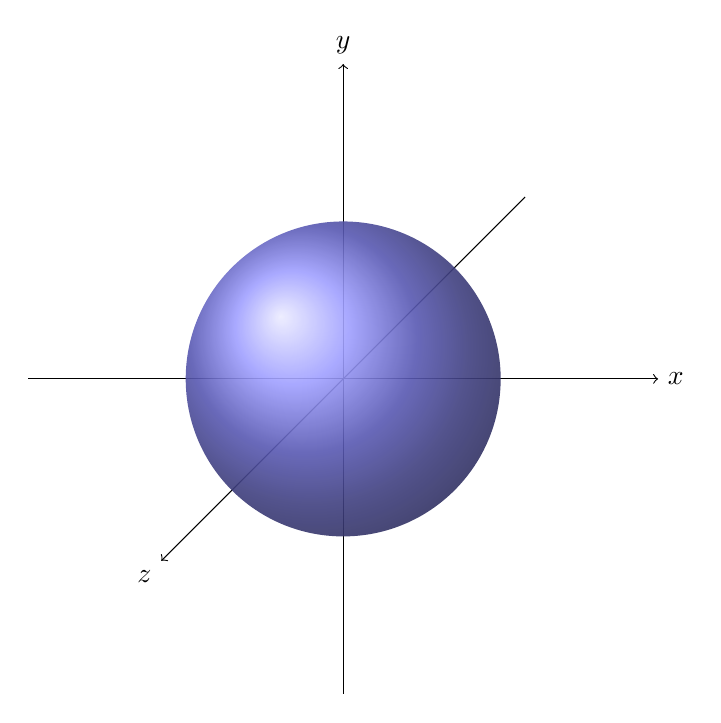
\begin{tikzpicture}[scale=2]
        % 坐标轴
        \draw[->] (-2,0,0) -- (2,0,0) node[right]{$x$};
        \draw[->] (0,-2,0) -- (0,2,0) node[above]{$y$};
        \draw[->] (0,0,-3) -- (0,0,3) node[below left]{$z$};
        
        % 绘制球体
        \shade[ball color=blue!50!white, opacity=0.9] (0,0,0) circle (1cm);
    \end{tikzpicture}
    $$
\end{example}
\begin{remark}
    仍然通过穿线积分法确定上下限,从原点引一条直线穿过平面,上下限即为后穿过的面和先穿过的面,角度由线的摆动范围
    决定。可以通过方程确定角度的上下限。
\end{remark}
\begin{remark}
    事实上,一元微积分中的换元公式仍然是一种坐标变换,只不过其雅可比行列式是一维行列式,即
    \begin{align*} 
        |J|=\begin{vmatrix}\frac{\mathrm dt}{\mathrm dx}\end{vmatrix}=\frac{\mathrm d t}{\mathrm d x}
    \end{align*} 
    因此,我们可以将一维的换元法统一到多元微积分中。这也就是最开始坐标变换的积分公式。
\end{remark}
\section{保守场是梯度场}
\subsection{保守场}
\begin{definition}
    定义保守场为,若积分路径两端点固定,那么积分值不变的场。
\end{definition}
这一定义表明了以下性质:
\begin{theorem} 
    \begin{align*} 
        \oint_C \nabla f\mathrm d r=0 \Rightarrow \nabla \times \vb{F}=0
    \end{align*}
\end{theorem}
\begin{remark} 
    但是,这个判据使用不够方便,因此我们需要一个容易的判据来判定一个场是否是保守场。
\end{remark}
\begin{theorem}
    对于向量场$\vb{F} = M \vb{i} + N \vb{j} + P \vb{k}$,那么若
    \begin{align*} 
        \frac{\partial M}{\partial y}=\frac{\partial N}{\partial x},\frac{\partial M}{\partial z}=\frac{\partial P}{\partial x},\frac{\partial N}{\partial z}=\frac{\partial P}{\partial y}
    \end{align*}
    则$\vb{F}$是保守场。
\end{theorem}
\begin{remark}
    该定理实际上等价于求导顺序可交换。该定理是一个充分必要条件。
\end{remark}
\subsection{保守场是梯度场}
\begin{theorem} 
    保守场是梯度场,也就是说
    \begin{align*} 
        \vb{F} =\nabla f 
    \end{align*}
    其中$f$是势函数。
\end{theorem}
\subsection{如何求解势函数} 
\begin{lemma} 
    我们已知向量场$\vb{F} = M \vb{i} + N \vb{j} + P \vb{k}$,我们可以通过以下步骤求解势函数:
    \begin{enumerate} 
        \item 求$\vb{F}$的梯度,得到$\vb{F} = \nabla f$;
        \item 然后,解微分方程得到$f(x,y,z)+C$
        \item 最后,通过常数确定函数。
    \end{enumerate}
\end{lemma}
\subsection{恰当微分形式} 
\begin{definition}
    定义恰当微分形式为
    \begin{align*} 
        \mathrm d f = M\mathrm d x + N\mathrm d y + P\mathrm d z = \frac{\partial f}{\partial x}\mathrm dx + \frac{\partial f}{\partial y}\mathrm dy + \frac{\partial f}{\partial z}\mathrm dz
    \end{align*}
    其中$M,N,P$为函数。
\end{definition}
\section{格林公式}
\subsection{格林公式}
我们在第九章介绍了两类曲线积分,接下来我们介绍闭区域与其边界的关系。
\begin{theorem}[格林公式]
函数$P(x,y)$,$Q(x,y)$在D上有连续一阶偏导数,L是D的光滑边界,则
\begin{align*}
    \iint_{D}\begin{vmatrix}\frac{\partial }m{\partial x}&\frac{\partial }{\partial y}\\P&Q\end{vmatrix}\mathrm d{x}\mathrm{d}y=\iint_{D}(\frac{\partial Q}{\partial x}-\frac{\partial P}{\partial y})\mathrm d{x}\mathrm{d}y=\oint_{L^{+}} P\mathrm d x+Q\mathrm d y
    =\oint_{L}\vb{F}\cdot \diff \vb{r}
\end{align*}
其中$L^{+}$为正向(逆时针)边界。若内部还有边界,保证区域总在前进方向的左边(如在右边,加上负号即可)即可。
\end{theorem}
\begin{remark}
函数$P,Q$可以被视为密度函数,其中$P$是$x$方向上的密度函数,$Q$为$y$方向上的密度函数。对于均匀面积,可以直接使用
$\iint_D \mathrm d A$,即$P=Q=1$。
\end{remark}
\paragraph{}该公式建立了区域积分与线积分之间的桥梁,从而使我们可以通过求解好求的一边得到积分结果。
\begin{remark}
    在很多情况下,积分路径的参数化是比较复杂的,因此我们可以考虑将积分使用格林公式化为面积分,从而简化计算。
\end{remark}
\begin{theorem}
    如果积分区域内存在内边界,那么满足
    \begin{align*} 
        \oint_C \vb{F}\cdot \diff \vb{r} - \sum_{i = 1}^n \oint_{C_i} \vb{F}\cdot \diff \vb{r} = \iint_D (\frac{\partial Q}{\partial x}-\frac{\partial P}{\partial y})\mathrm d{x}\mathrm{d}y
    \end{align*}
\end{theorem}   
\subsection{环量密度}
\begin{definition}
    定义平面上环量密度为
    \begin{align*} 
        \omega = P\mathrm d x - Q\mathrm d y
    \end{align*} 
    其中$P,Q$为密度函数。记为$\mathrm{curl}\vb{F}\cdot  \vb{k}$。
\end{definition}
\section{斯托克斯公式}
\subsection{参数曲面}
\begin{definition} 
    定义参数曲面为
    \begin{align*} 
        \vb{r}(u,v) = x(u,v)\vb{i} + y(u,v)\vb{j} + z(u,v)\vb{k}
    \end{align*} 
    其中$u,v$为参数。
\end{definition}
\begin{definition}[光滑] 
    定义光滑曲面为,曲面上每一点都有一个唯一的切平面。也就是说,曲面上偏导数存在且连续,且其叉乘不为零。
\end{definition}
\begin{theorem} 
    对于参数曲面$\vb {r}(u,v) = x(u,v)\vb{i} + y(u,v)\vb{j} + z(u,v)\vb{k}$的面积,我们有
    \begin{align*} 
        S = \iint_D |\vb{r}_u\times \vb{r}_v|\diff v \diff u
    \end{align*}
    其中$\vb{r}_u$和$\vb{r}_v$分别为参数曲面在$u,v$方向上的偏导数。
\end{theorem}
\begin{remark}
    这里的叉乘实际上是计算微小区域上平行四边形的面积,因此我们可以将其视为面积元素。
\end{remark}
\begin{lemma}[隐曲面引理]
    对于隐平面$F(x,y,z)=c$,那么该曲面面积为
    \begin{align*} 
        \iint_R \frac{|\nabla F|}{|\nabla F\cdot \vb{p}|}\diff A
    \end{align*} 
    其中$\vb{p}$为垂直于积分区域$R$的向量。
\end{lemma}
\begin{lemma}[$z=f(x,y)$的面积] 
    对于曲面$z=f(x,y)$,那么该曲面面积为
    \begin{align*} 
        S = \iint_D \sqrt{1+(\frac{\partial f}{\partial x})^2+(\frac{\partial f}{\partial y})^2}\diff A
    \end{align*}
    其中$D$为投影区域。
\end{lemma}
\begin{theorem}[在曲面上对标量场积分]
    对于曲面$S$上的标量场$f(x,y,z)$,那么该曲面上的积分为
    \begin{align*} 
        \iint_S f(x,y,z)\diff S = \iint_D f(x(u,v),y(u,v),z(u,v))|\vb{r}_u\times \vb{r}_v|\diff u\diff v
    \end{align*}
\end{theorem}
\begin{remark} 
    该公式实际上是对微元乘上了一个密度函数,其余的公式也同样是对面积元乘以一个密度函数。
\end{remark}
\subsection{斯托克斯公式}
\begin{definition}[曲面上向量场积分]
    定义对于曲面$S$上的向量场$\vb{F}$的积分为
    \begin{align*} 
        \iint_S \vb{F}\cdot \vb{n}\diff S = \iint_S \vb{F}\cdot \frac{\vb{r}_u\times\vb{r}_v}{|\vb{r}_u\times\vb{r}_v|}\diff S
    \end{align*} 
\end{definition}
当我们的考量对象从二维场变化为三维场,我们需要更强的数学工具来计算,通过推导,我们可以用格林公式推导斯托克斯公式:
\begin{theorem}[斯托克斯公式]函数$P(x,y,z),Q(x,y,z),R(x,y,z)$在S上有连续一阶偏导数,L是D的光滑边界,则对于曲面$f(x,y,z)=0$
\begin{align*}
    \iint_S \nabla \times F \diff S=\iint_{S}\begin{vmatrix}\cos \alpha&\cos \beta&\cos\gamma\\\frac{\partial}{\partial x}&\frac{\partial}{\partial y}&\frac{\partial}{\partial z}\\P&Q&R\end{vmatrix}\mathrm dS=\oint_{L^{+}} P\mathrm d x+Q\mathrm d y+R\mathrm d z
\end{align*}
并且令$\cos\alpha =\pm \frac{p}{\sqrt{1+p^2+q^2}},\cos\beta =\pm \frac{q}{\sqrt{1+p^2+q^2}},\cos\gamma =\pm \frac{1}{\sqrt{1+p^2+q^2}}$,其中$p=\frac{\partial f}{\partial x},q=\frac{\partial f}{\partial y}.$
\end{theorem}
\begin{remark}
将公式写为行列式以后,我们不难发现斯托克斯公式的特殊情况就是格林公式。
\end{remark}
\section{高斯公式}
更进一步,我们有
\begin{theorem}[高斯公式]
\begin{align*}
    \iiint_{\Omega}(\frac{\partial Q}{\partial x}+\frac{\partial P}{\partial y}+\frac{\partial R}{\partial z})\mathrm d{x}\mathrm{d}y\mathrm d z=\iint_{\Sigma^{+}} P\mathrm d y\mathrm d z+Q\mathrm d x\mathrm d z+R\mathrm d x\mathrm d y
\end{align*}
$\Sigma^{+}$表示法向量指向闭合曲面外侧。
\end{theorem}
\section{一般形式的斯托克斯公式}
\begin{theorem}[斯托克斯公式一般形式]
\begin{align*}
    \int_{\partial\Omega}\omega =\int_{\Omega}\mathrm d \omega
\end{align*}
其中$\omega$为微分形式,$\mathrm d\omega$为$\omega$的外微分,$\Omega$为n维流形的某个区域,$\partial\Omega$为其边界。
\end{theorem}
\begin{remark}
把这个公式放在这里是因为它很漂亮。
定义微分形式 $\omega$
\begin{align*} 
    \omega = \sum_{1<i_1<i_2<i_3<...<i_n\leq n} f_{i_1,i_2,\cdots,i_n}\mathrm d x_{i_1}\wedge \mathrm d x_{i_2}\wedge \cdots \wedge \mathrm d x_{i_n}
\end{align*}
其中,定义外微分
\begin{align*} 
    \diff \omega = \sum_{1<i_1<i_2<i_3<...<i_n\leq n} (\sum_{i=1}^n\frac{\partial f_{i_1,i_2,\cdots,i_n}}{\partial x_j}\mathrm d x_j) \mathrm d x_{i_1}\wedge \mathrm d x_{i_2}\wedge \cdots \wedge \mathrm d x_{i_n}
\end{align*}
其中$\wedge$表示外积。我们可以将其视为一个多元函数的外微分。
\end{remark}
\begin{lemma}[Poncar\'{e}'s Lemma]
    \begin{align*}
    \diff^2 = 0
    \end{align*}
\end{lemma}
\section{求物体的质心}
\subsection{物体的质心公式}
\begin{theorem}
    一个物体的质心处于(以x方向为例)
    \begin{align*} 
        \overline{x} = \frac{\iiint x \mathrm d m}{\iiint \mathrm dm}
    \end{align*} 
\end{theorem}
\begin{remark}
    事实上,质心就是坐标对质量的加权平均。
\end{remark}

\chapter{实分析入门}
\section{集合}
\section{勒贝格测度}
\section{勒贝格积分}
\chapter{复分析入门}
\chapter{泛函分析入门}

\end{document}